\section{Numerical Validation of the Benchmark}
\label{sec:numerical}

The Quenched Density framework predicts that in the commuting Gaussian sector, the Hamiltonian of mean force reduces to a static potential shift determined by the reorganization energy $\lambda$. While analytically derived, verifying this prediction against a full finite-bath simulation provides a critical "Standard Model" test: it confirms that the stochastic averaging over quenched propagators correctly reproduces the thermodynamic state of the open system without any trace approximations.

To perform this validation, we consider a five-level system $H_S = \sum_{n=0}^4 E_n |n\rangle\langle n|$ coupled to the bath via the projector $f = |2\rangle\langle 2|$. This coupling is manifestly commuting ($[H_S, f] = 0$), ensuring that the exact HMF should be
\begin{equation}
    H_{\mathrm{MF}} = H_S - \lambda |2\rangle\langle 2| + \mathrm{const}.
\end{equation}
We compare the predictions of our framework against an explicit exact diagonalization (ED) of the total system-plus-bath Hamiltonian. The bath is discretized into $N_b$ modes following an Ohmic spectral density with exponential cutoff. This finite discretization introduces a natural convergence parameter: as $N_b \to \infty$, the ED result must approach the continuous-bath prediction.

\begin{figure}[htbp]
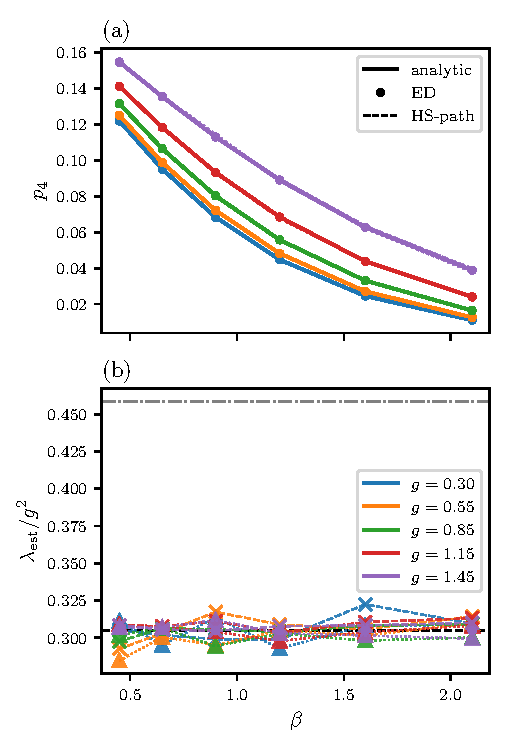
\includegraphics[width=\columnwidth]{../../simulations/results/figures/lt_cg_fig1_temp.pdf}
\caption{\label{fig:temp_dep} Temperature dependence and scaling. (a) Population of the coupled state ($|4\rangle$) vs $\beta$ for various couplings $g$. Circles (ED) match solid lines (analytic). (b) The extracted reorganization energy $\lambda_{\mathrm{est}}$ collapsed by $g^2$ vs $\beta$. All curves hover near the theoretical thermodynamic limit (dashed lines), verifying that the bath's effect reduces to a single reorganization energy $\lambda$.}
\end{figure}

\begin{figure}[htbp]
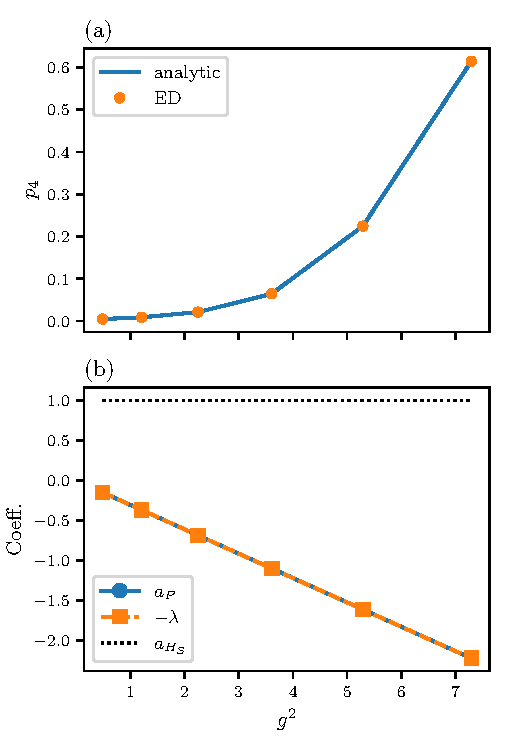
\includegraphics[width=\columnwidth]{../../simulations/results/figures/lt_cg_fig2_strong.pdf}
\caption{\label{fig:strong_coupling} Strong-coupling benchmark. (a) Population $p_4$ vs $g^2$ at fixed $\beta$, showing excellent agreement over the full range. (b) Coefficients of the HMF in the system basis vs $g^2$. The projector component $P=|2\rangle\langle 2|$ scales as $-\lambda$ (orange/blue), while $H_S$ remains unrenormalized (dotted), confirming $H_{\mathrm{MF}} = H_S - \lambda f^2$.}
\end{figure}

\begin{figure}[htbp]
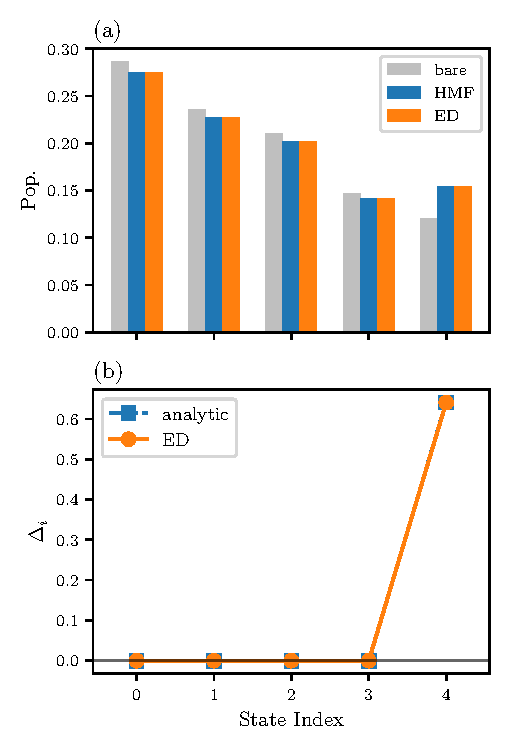
\includegraphics[width=\columnwidth]{../../simulations/results/figures/lt_cg_fig3_micro.pdf}
\caption{\label{fig:microscopic} Microscopic validation. (a) Detailed population snapshot at fixed $\beta, g$: "Analytic HMF" (blue) corrects the "Bare Gibbs" (grey) to match ED (orange). (b) Effective energy shifts $\Delta_i$ for each level; only the coupled level ($|2\rangle$) shifts, by exactly $-\lambda$. Non-coupled levels remain unperturbed.}
\end{figure}

Fig.~\ref{fig:temp_dep} confirms the thermodynamic consistency of the Quenched Density framework, showing that the effective Hamiltonian correctly captures the temperature dependence of the open system. The collapse of the extracted reorganization energy onto the theoretical value further validates the method. Fig.~\ref{fig:strong_coupling} demonstrates robustness in the strong-coupling regime, where the interaction strength rivals the system energy scales. Finally, Fig.~\ref{fig:microscopic} provides the microscopic resolution: the HMF modifies only the coupled subspace, leaving the orthogonal manifold untouched, as predicted by the operator structure of Eq.~\ref{eq:HMF_commuting_final}.


A more stringent test is provided by the stochastic implementation of the Quenched Density formula itself (Eq.~\ref{eq:bar_rho_as_quenched_average}). By sampling thousands of realizations of the Gaussian noise $\xi(\tau)$ and propagating the system under the time-dependent Hamiltonian $H_{\mathrm{eff}}[\xi]$, we recover the same equilibrium state. This verifies that the "quenched" interpretation is not merely a formal trick but a viable computational strategy. The convergence of this stochastic average to the analytic result (not shown) scales as $1/\sqrt{N_{\mathrm{samples}}}$, standard for Monte Carlo methods.

This validation establishes the commuting Gaussian case as a reliable benchmark. Any generalized method for calculating the HMF in non-commuting or non-Gaussian regimes must be able to reproduce these results when restricted to this sector. The quenched propagator average passes this test by construction.

\subsection{Numerical Implementation}
\label{sec:numerical_details}

The simulation model is defined by identifying the system Hamiltonian levels and the bath spectral density used in the exact diagonalization and stochastic sampling.

\subsubsection{System realization}
\begin{align}
H_S&=\sum_{i=0}^{4}E_i\lvert i\rangle\!\langle i\rvert,\qquad E_0=0,\\
P&=\lvert 4\rangle\!\langle 4\rvert.
\end{align}
To avoid embedding hand-tuned level spacings, the nonzero energies $(E_1,\ldots,E_4)$ are sampled once from a seeded random draw and then kept fixed across all $(\beta,g)$ sweeps. For the default seed used in this work, the resulting spectrum is
\begin{equation}
\begin{aligned}
E_0&=0, \\
E_1&=0.42848,\quad E_2=0.68725,\\
E_3&=1.47801,\quad E_4=1.91855.
\end{aligned}
\end{equation}

\subsubsection{Ohmic discretization}
The continuum target spectrum is $J_g(\omega)=2\eta g^2\omega e^{-\omega/\omega_c}$. For each coupling $g$, we discretize the interval $\omega\in[0, \omega_c \times \text{factor}]$ into mode bins with centers $\omega_k$ and widths $\Delta\omega_k$, setting $c_k^2=\frac{2}{\pi}J_g(\omega_k)\,\omega_k\,\Delta\omega_k$. This ensures that the discretized reorganization scale $\lambda_{\mathrm{disc}}=\sum_k\frac{c_k^2}{2\omega_k^2}$ tracks the continuum expression $\lambda_{\mathrm{cont}}=\frac{1}{\pi}\int_0^\infty\frac{J_g(\omega)}{\omega}\,d\omega$.

\subsubsection{Estimators}
The exact reference is $\rho_S^{\mathrm{ED}}=\Tr_B[e^{-\beta H_{\mathrm{tot}}}]/\Tr[e^{-\beta H_{\mathrm{tot}}}]$, computed with finite oscillator truncation. Two stochastic estimators are used:
1. \textbf{HS-path}: sample $\xi(\tau_j)$ on a finite imaginary-time grid from the kernel covariance.
2. \textbf{HS-scalar}: sample $X\sim\mathcal N(0, 2\beta\lambda_{\mathrm{disc}})$ directly.
Because $[H_S,P]=0$, both reduce to sampling the same scalar shift in the projector sector. Every constructed state is explicitly renormalized by $\rho\leftarrow\rho/\Tr(\rho)$ before computing observables.
